\documentclass[border=10pt]{standalone}

\usepackage{tikz}
\usepackage{tikzsymbols}
\usetikzlibrary{calc,patterns,shapes.geometric}

\def\centerarc[#1](#2)(#3:#4:#5){\draw[#1] ($(#2)+({#5*cos(#3)},{#5*sin(#3)})$) arc (#3:#4:#5);}

\begin{document}
	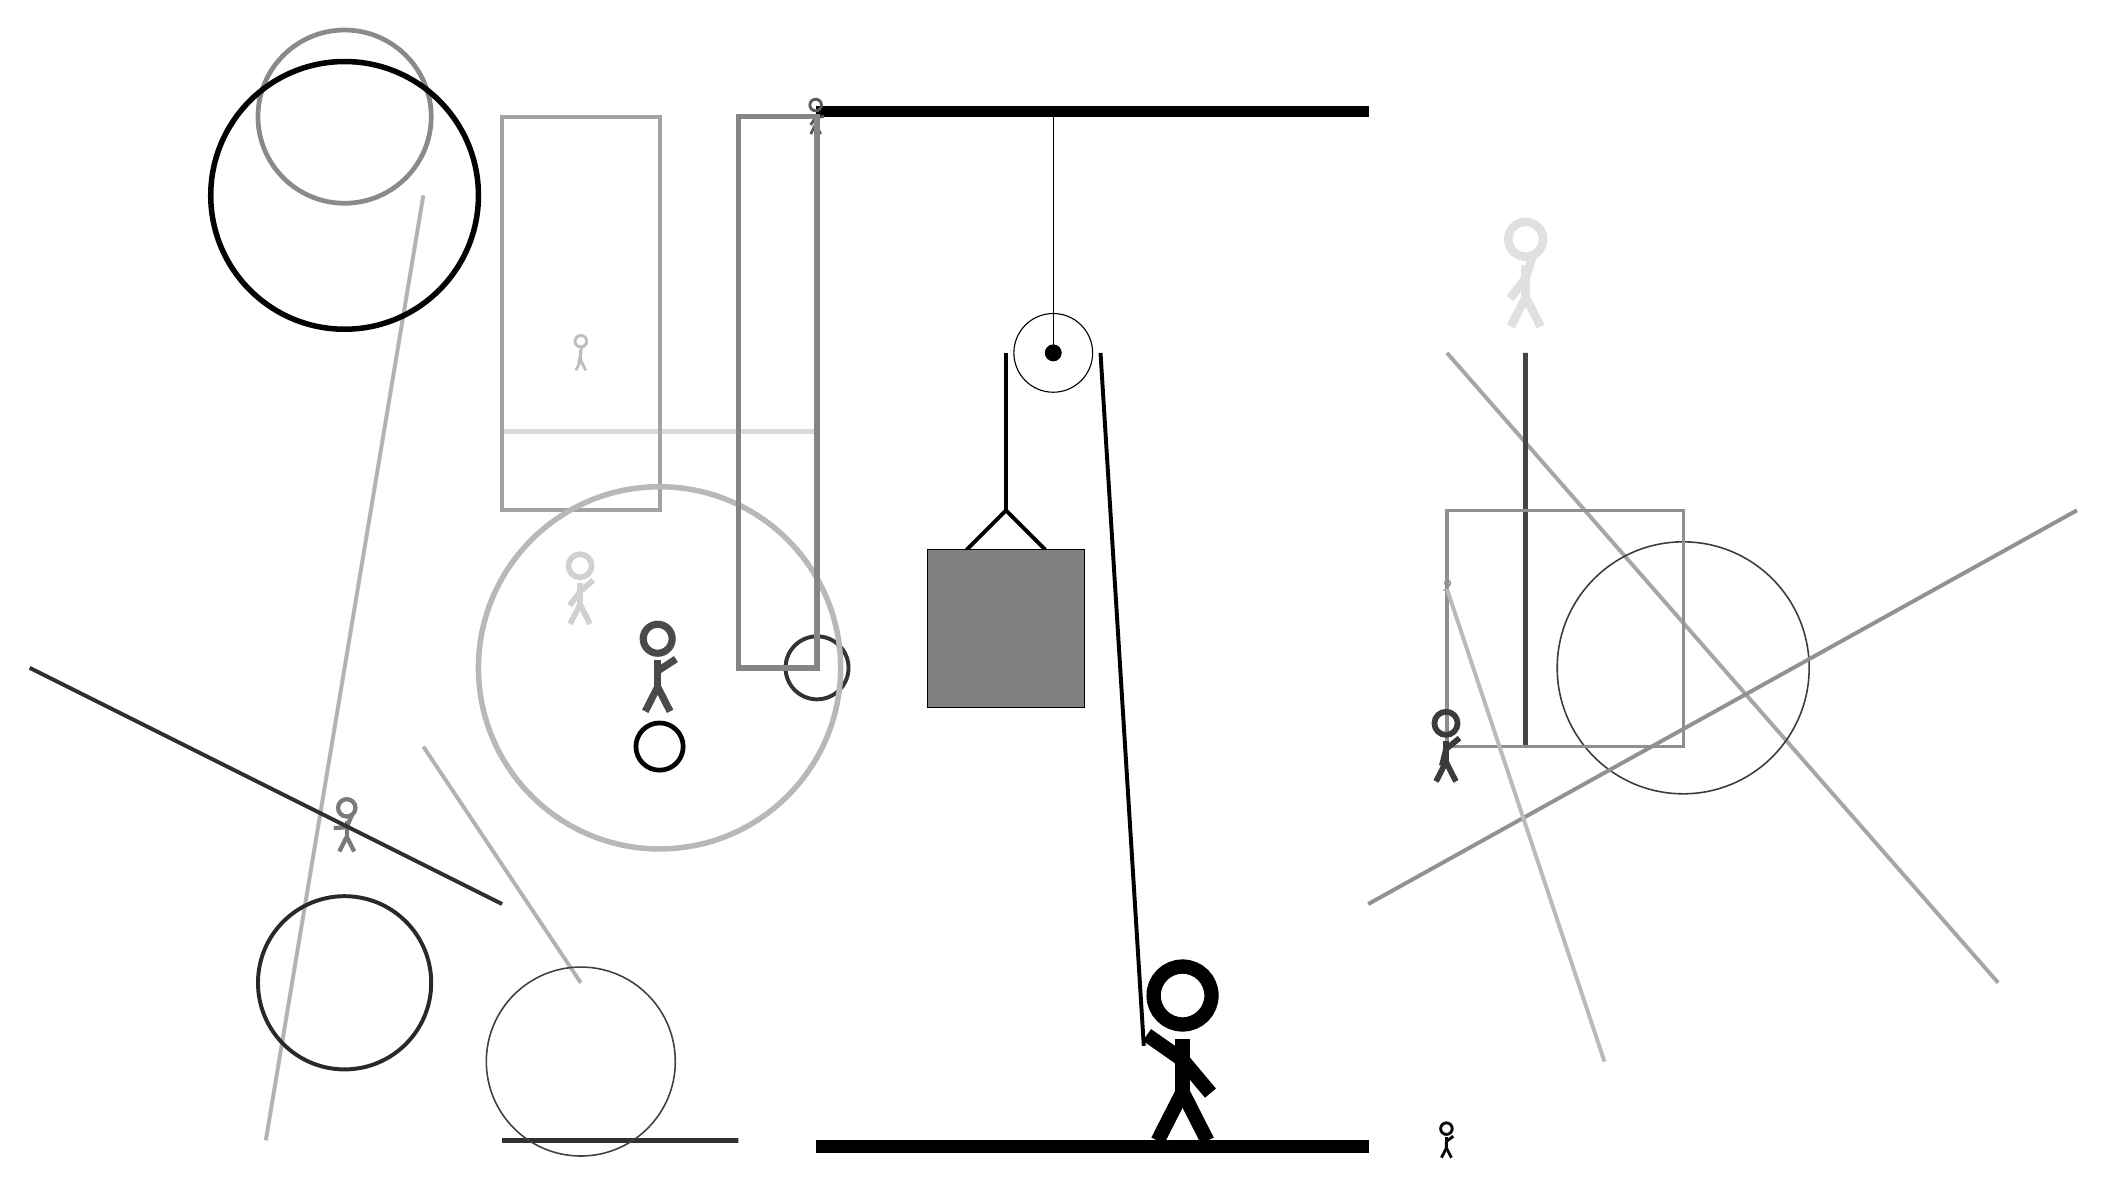
\begin{tikzpicture}
		%%%%% START %%%%%
		
		\draw[fill=black] (-2, 10) rectangle (5, 10.125);
		
		\draw (1, 7) circle (0.5);
		\draw[fill=black] (1, 7) circle (0.1);
		\draw (1, 10) -- (1, 7);
		
		\draw[line width=0.5mm] (-0.1, 4.5) -- (0.4, 5.0) -- (0.9, 4.5);
		\draw[fill=black!50] (-0.6, 4.5) rectangle (1.4, 2.5);
		
		\draw[line width=0.5mm] (0.4, 7) -- (0.4, 5.0);
		\centerarc[line width=0.5mm](1, 7)(0:180:0.6);
		\draw[line width=0.5mm](1.6, 7) -- (2.15, -1.8);
		
		\node at (2.6, -1.9) {\Strichmaxerl[10][-35][-50]};
		
		\node[line width=0.2mm, color=black!41] at (6, 4) {\Strichmaxerl[1][7][88]};
		
		\draw[line width=0.5mm, color=black!35](6, 7) -- (13, -1);
		\draw[line width=0.7mm, color=black!81] (-3, -3) rectangle (-6, -3);
		\draw[line width=0.7mm, color=black!15] (-2, 6) rectangle (-6, 6);
		
		\node[line width=0.4mm, color=black!97] at (6, -3) {\Strichmaxerl[2][89][38]};
		
		\draw[line width=0.7mm, color=black!73] (7, 7) rectangle (7, 2);
		\node[line width=0.6mm, color=black!52] at (-8, 1) {\Strichmaxerl[3][4][67]};
		
		\node[line width=0.4mm, color=black!65] at (-2, 10) {\Strichmaxerl[2][54][11]};
		\draw [line width=0.6mm, color=black!46](-8, 10) circle (1.1);
		\draw [line width=0.5mm, color=black!80](-2, 3) circle (0.4);
		
		\draw [line width=0.2mm, color=black!77](9, 3) circle (1.6);
		\draw[line width=0.5mm, color=black!43](5, 0) -- (14, 5);
		\draw[line width=0.5mm, color=black!30](-7, 2) -- (-5, -1);
		\draw[line width=0.5mm, color=black!36] (-4, 5) rectangle (-6, 10);
		\node[line width=0.7mm, color=black!18] at (-5, 4) {\Strichmaxerl[4][53][41]};
		\draw[line width=0.4mm, color=black!44] (6, 5) rectangle (9, 2);
		
		\draw [line width=0.7mm, color=black!28](-4, 3) circle (2.3);
		
		\draw[line width=0.5mm, color=black!30](-7, 9) -- (-9, -3);
		\node[line width=0.7mm, color=black!12] at (7, 8) {\Strichmaxerl[6][53][72]};
		
		\node[line width=0.4mm, color=black!77] at (6, 2) {\Strichmaxerl[4][76][39]};
		\draw [line width=0.7mm, color=black!99](-8, 9) circle (1.7);
		\draw [line width=0.5mm, color=black!84](-8, -1) circle (1.1);
		\draw[line width=0.7mm, color=black!48] (-2, 3) rectangle (-3, 10);
		\draw [line width=0.6mm, color=black!99](-4, 2) circle (0.3);
		\node[line width=0.2mm, color=black!26] at (-5, 7) {\Strichmaxerl[2][76][86]};
		
		\draw [line width=0.6mm, color=black!97](6, 4) circle (0.0);
		\draw[line width=0.5mm, color=black!27](8, -2) -- (6, 4);
		\draw [line width=0.2mm, color=black!75](-5, -2) circle (1.2);
		
		\draw[line width=0.5mm, color=black!81](-6, 0) -- (-12, 3);
		\draw [line width=0.2mm, color=black!100](10, 3) circle (0.0);
		\node[line width=0.5mm, color=black!71] at (-4, 3) {\Strichmaxerl[5][90][33]};
		
		
		\draw[fill=black] (-2, -3) rectangle (5, -3.15);
		
		%%%%% END %%%%%
	\end{tikzpicture}
\end{document}